\section{A toolkit for interactive data provenance}
\label{sec:toolkit}

Having established this core bidirectional analysis, we now show how it can form the basis of a toolkit for automatically enriching data visualisations and other structured outputs with affordances that allow a user to interactive explore their relationship to data, and to each other. We also contrast the proposed approach with prior work on program slicing based on Galois connections.

\begin{figure}
   \begin{subfigure}{0.53\textwidth}
      {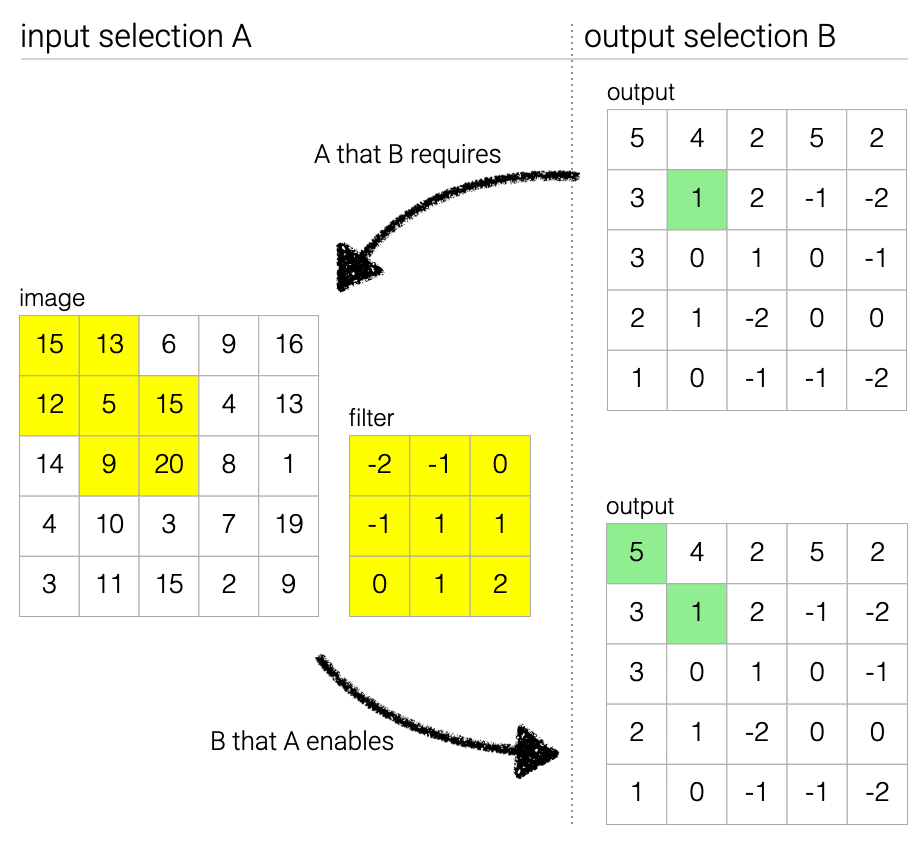
\includegraphics[scale=0.4]{fig/example/4-relations-1.png}}
      \vspace{2mm}
      \caption{Galois dependency $(\evalBwdF{T}, \evalFwdF{T})$}
      \label{fig:example:convolve-viz:galois-dependency}
   \end{subfigure}
   \begin{subfigure}{0.46\textwidth}
      {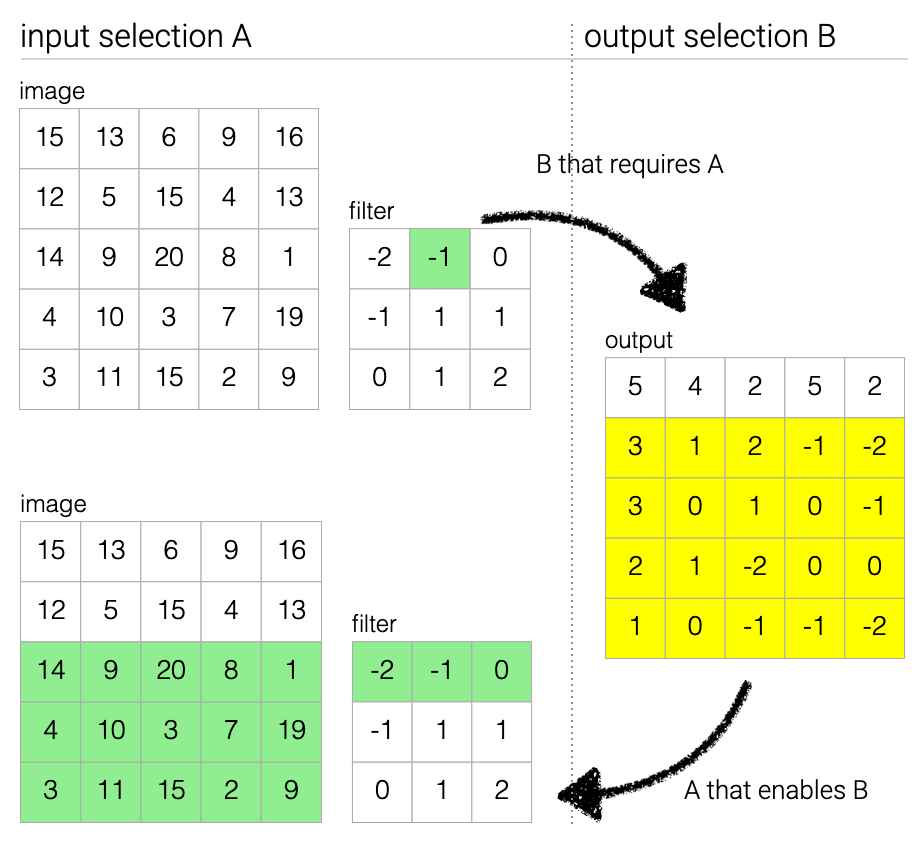
\includegraphics[scale=0.4]{fig/example/4-relations-2.png}}
      \vspace{2mm}
      \caption{De Morgan dual $(\dual{\evalFwdF{T}}, \dual{\evalBwdF{T}})$}
      \label{fig:example:convolve-viz:de-morgan-dual}
   \end{subfigure}
   \caption{Upper and lower pairs are dual; left and right pairs are adjoint}
   \label{fig:example:convolve-viz}
\end{figure}


The fine-grained relationship between visual elements and data intuitively has the flavour of an adjunction. Given a data selection, we might ask whether it contains the data required to reconstruct --- whether it is \emph{sufficient for} --- a given part of the chart. Dually, given a visual selection, we might ask whether it is small enough to be generated by a given data selection. Additionally we might wonder whether there are minimal/maximal solutions to these problems.

These considerations points towards \emph{Galois connections} as a way of formalising these dynamic input-output relations, and indeed in the program slicing literature, dynamic analyses based on Galois connections have been developed for pure functional programs~\cite{perera12a}, functional programs with effects~\cite{ricciotti17}, and \piCalculus~\cite{perera16d}. These ``Galois slicing'' techniques have the flavour of what we need, but are unable to compute the kind of sufficiency relation we just outlined. To see the problem, we briefly outline how Galois slicing works. The idea is generalise the notion of program and value to \emph{program slices} and \emph{value slices}, program and values where some subexpressions have been replaced by hole $\hole$. A program slice ``evaluates'' to a \emph{value slice}, a value where some subvalues have been replaced by $\hole$, and dual to this, a value slice induces a (minimal) program slice. One can then extend this basic framework to focus on

The problem with this approach is that it does not readily extend to a notion of selection where the part of the output of interest is not a prefix of the output, but rather a prefix of some subtree. For example, if we consider the following program, which has the value \lstinline{(0.4, 0.6)}:

\begin{figure}
   \small
   \begin{centering}
      \begin{subfigure}{0.45\textwidth}
         {\lstinputlisting[language=Fluid,escapeinside={(*@}{@*)}]{other-src/diff-slicing-0.example}}
      \caption{Original program}
      \label{fig:example:diff-slicing:original}
      \end{subfigure}
      \begin{subfigure}{0.45\textwidth}
         {\lstinputlisting[language=Fluid,escapeinside={(*@}{@*)}]{other-src/diff-slicing-2.example}}
      \caption{Backward slice for \kw{(0.4, $\hole$)}}
      \label{fig:example:diff-slicing:subtree}
      \end{subfigure}
      \\
      \begin{subfigure}{0.45\textwidth}
         {\lstinputlisting[language=Fluid,escapeinside={(*@}{@*)}]{other-src/diff-slicing-1.example}}
      \caption{Backward slice for spine \kw{($\hole$, $\hole$)}}
      \label{fig:example:diff-slicing:spine}
      \end{subfigure}
      \begin{subfigure}{0.45\textwidth}
         {\lstinputlisting[language=Fluid,escapeinside={(*@}{@*)}]{other-src/diff-slicing-3.example}}
      \caption{Differential backward slice for \kw{(\codeSelTwo{0.4}, $\hole$)}}
      \label{fig:example:diff-slicing:differential}
      \end{subfigure}
   \end{centering}
   \vspace{-2mm}
   \caption{Differential Galois slicing selects input (blue) needed \emph{only} for selected output (green)}
   \label{fig:example:diff-slicing}
\end{figure}


\noindent Because differential slicing includes a program part if is needed \emph{only} by the selected output, in general it underapproximates the parts actually needed for the selected output. In this example, \lstinline{2} and \lstinline{3} are both needed to compute the spine containing the subtree of interest, and so the differential slice does not include them. Differential slicing based on tree prefixes is thus not a suitable technique for computing data dependencies.

\subsection{Linking cognate visualisations}

Intuitively, selections in cognate visualisations can be linked through their common data, which also a bidirectional quality: one must consider how dependencies flow ``backward'' from selections in one chart to a selection $S$ in the underlying data, and then ``forward'' from the selected data $S$ to a corresponding selection in the other chart. However the flavour of the forward dependency differs from the notion of ``sufficiency'' outlined in the previous section: to determine the related parts of the other chart, we must consider not what the data selection $S$ is \emph{sufficient} for, but what it is \emph{necessary} for: those parts of the other visualisation that depend on $S$.

\todo{Introduce negation and the other Galois connection that can be derived from negation.}

\begin{figure}[H]
   \small
   \lstinputlisting[language=Fluid]{fluid/convolution.fld.mod}
   \caption{Matrix convolution, with three methods for dealing with boundaries}
\end{figure}

\begin{figure}[H]
   \small
   \lstinputlisting[language=Fluid]{fluid/conv-extend.fld.mod}
   \caption{Convolving example matrix with supplied filter and choice of boundary method}
\end{figure}

